\chapter{The Bloch sphere and single-qubit gates}\label{ch:bloch}

The geometrical representation of a two-level system as a vector on a sphere appeared as the \emph{pseudospin} representation of
Feynman, Vernon and Hellwarth \cite{FVH1957}, building on F.~Bloch's equations for nuclear spins (1946). For light, the same
construction is the Poincaré sphere (H.~Poincaré, 1892) of polarization states.

\section{Pauli matrices}\label{sec:pauli}
\subsection{Algebra}
The identity and the Pauli matrices are
\begin{equation}
  \sigma_0=\begin{pmatrix}1&0\\0&1\end{pmatrix},\quad
  \sigma_x=\begin{pmatrix}0&1\\1&0\end{pmatrix},\quad
  \sigma_y=\begin{pmatrix}0&-\ii\\ \ii&0\end{pmatrix},\quad
  \sigma_z=\begin{pmatrix}1&0\\0&-1\end{pmatrix}.
\end{equation}
They are Hermitian, unitary and traceless (except $\sigma_0$), and square to the identity. Their products follow from a single identity,
\begin{equation}\label{eq:pauliproduct}
  \sigma_j\sigma_k=\delta_{jk}\,I+\ii\sum_l\varepsilon_{jkl}\sigma_l,\qquad j,k,l\in\{x,y,z\},
\end{equation}
where $\varepsilon_{jkl}$ is the Levi-Civita symbol. For example $\sigma_x\sigma_y=\ii\sigma_z$; check it by multiplying the matrices.
Consequences:
\begin{equation}
  [\sigma_j,\sigma_k]=2\ii\varepsilon_{jkl}\sigma_l,\qquad\{\sigma_j,\sigma_k\}=2\delta_{jk}I,\qquad
  (\vec a\cdot\vec\sigma)(\vec b\cdot\vec\sigma)=(\vec a\cdot\vec b)\,I+\ii(\vec a\times\vec b)\cdot\vec\sigma.
\end{equation}
The last identity, valid for real vectors, follows by multiplying \cref{eq:pauliproduct} by $a_jb_k$ and summing. In particular
$(\vec n\cdot\vec\sigma)^2=I$ for a unit vector $\vec n$, so the eigenvalues of $\vec n\cdot\vec\sigma$ are $\pm1$.

\subsection{Decomposition of a $2\times2$ Hamiltonian}
The four matrices are orthogonal for the Hilbert--Schmidt scalar product $\langle A,B\rangle=\tr(A^\dagger B)$:
\begin{equation}
  \tr(\sigma_\alpha\sigma_\beta)=2\delta_{\alpha\beta},\qquad\alpha,\beta\in\{0,x,y,z\},
\end{equation}
which follows from \cref{eq:pauliproduct} and $\tr\sigma_l=0$. Four orthogonal (hence linearly independent) elements of the
four-dimensional space of $2\times2$ complex matrices form a basis. Any matrix can therefore be written
\begin{equation}
  H=\begin{pmatrix}a&b\\c&d\end{pmatrix}=h_0\sigma_0+h_x\sigma_x+h_y\sigma_y+h_z\sigma_z
  =\begin{pmatrix}h_0+h_z&h_x-\ii h_y\\h_x+\ii h_y&h_0-h_z\end{pmatrix},\qquad h_\alpha=\tfrac12\tr(H\sigma_\alpha),
\end{equation}
where the formula for the coefficients is obtained by multiplying by $\sigma_\beta$ and taking the trace. Identifying the elements,
\begin{equation}
  h_0=\frac{a+d}2,\quad h_z=\frac{a-d}2,\quad h_x=\frac{b+c}2,\quad h_y=\frac{\ii(b-c)}2.
\end{equation}
For a Hermitian matrix, $a,d\in\R$ and $c=b^*$, so all four coefficients are real: $h_x=\operatorname{Re}b$, $h_y=-\operatorname{Im}b$.
Writing $\vec h=(h_x,h_y,h_z)$,
\begin{equation}\label{eq:Hpauli}
  H=h_0\sigma_0+\vec h\cdot\vec\sigma,\qquad
  E_\pm=h_0\pm|\vec h|=\frac{a+d}2\pm\sqrt{\left(\frac{a-d}2\right)^2+|b|^2}.
\end{equation}
The eigenvalues follow from $(\vec h\cdot\vec\sigma)^2=|\vec h|^2I$. The term $h_0\sigma_0$ adds only a global phase $\e^{-\ii h_0t/\hbar}$ and does not
affect the dynamics. \emph{The physics of a two-level system is entirely contained in a three-dimensional real vector $\vec h$}: its length gives
the level splitting $2|\vec h|$, its direction gives the eigenstates. For example, for $a=d=0$, $b=c=\hbar\omega/2$, we get
$\vec h=(\hbar\omega/2,0,0)$, $E_\pm=\pm\hbar\omega/2$, i.e.\ $H=\frac{\hbar\omega}2\sigma_x$.

\section{The Bloch sphere}
\subsection{Parametrization of a pure state}
A qubit state $\ket\psi=\alpha\ket0+\beta\ket1$ has four real parameters. Normalization removes one and the global phase another, leaving two,
which can be taken as angles on a sphere. Choosing the global phase so that $\alpha$ is real and non-negative,
\begin{equation}\label{eq:blochstate}
  \ket\psi=\cos\frac\theta2\ket0+\e^{\ii\varphi}\sin\frac\theta2\ket1,\qquad\theta\in[0,\pi],\ \varphi\in[0,2\pi).
\end{equation}
The original notes write the equivalent form $(\cos\frac\theta2\e^{-\ii\varphi},\sin\frac\theta2)^T$, which differs by the global phase
$\e^{-\ii\varphi}$ (and describes the same physical state). The point of the unit sphere with polar angle $\theta$ and azimuth $\varphi$,
\begin{equation}
  \vec n=(\sin\theta\cos\varphi,\ \sin\theta\sin\varphi,\ \cos\theta),
\end{equation}
is the \emph{Bloch vector}. The north pole is $\ket0$, the south pole $\ket1$, the equator contains the equal superpositions
$\ket\pm=(\ket0\pm\ket1)/\sqrt2$ ($\pm x$) and $\ket{\pm\ii}=(\ket0\pm\ii\ket1)/\sqrt2$ ($\pm y$).

\begin{proposition}\label{prop:blochvector}
The Bloch vector is the vector of mean values of the Pauli matrices, $\vec n=\mel\psi{\vec\sigma}\psi$, and $\ket\psi$ is the eigenvector of
$\vec n\cdot\vec\sigma$ with eigenvalue $+1$.
\end{proposition}
\begin{proof}
With $c=\cos\frac\theta2$, $s=\sin\frac\theta2$:
$\expval{\sigma_z}=c^2-s^2=\cos\theta$;
$\expval{\sigma_x}=\alpha^*\beta+\beta^*\alpha=2cs\cos\varphi=\sin\theta\cos\varphi$;
$\expval{\sigma_y}=-\ii\alpha^*\beta+\ii\beta^*\alpha=2cs\sin\varphi=\sin\theta\sin\varphi$.
For the second statement,
$\vec n\cdot\vec\sigma=\begin{pmatrix}\cos\theta&\sin\theta\e^{-\ii\varphi}\\ \sin\theta\e^{\ii\varphi}&-\cos\theta\end{pmatrix}$, and
the first component of $(\vec n\cdot\vec\sigma)\ket\psi$ is $\cos\theta\,c+\sin\theta\,s=c(\cos\theta+2s^2)=c$, using
$\sin\theta=2sc$ and $\cos\theta=1-2s^2$; the second component is checked in the same way.
\end{proof}

\paragraph{Why half angles?} Orthogonal states, $\braket{\psi}{\psi'}=0$, are at \emph{antipodal} points of the sphere ($\theta'=\pi-\theta$,
$\varphi'=\varphi+\pi$): the angle on the sphere is twice the ``angle'' $\arccos|\braket\psi{\psi'}|$ in Hilbert space. Indeed
\begin{equation}\label{eq:overlapbloch}
  |\braket\psi{\psi'}|^2=\frac{1+\vec n\cdot\vec n'}2=\cos^2\frac{\Theta}2,
\end{equation}
where $\Theta$ is the angle between the Bloch vectors (proof: use \cref{prop:blochvector} and the projector \cref{eq:projector} below).
For photons this explains the factor two between polarization angles and angles on the Poincaré sphere (\cref{sec:photonic}).

\begin{figure}[h]\centering
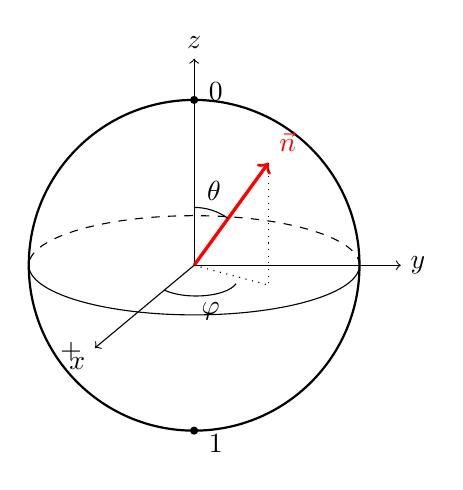
\begin{tikzpicture}[scale=2.1]
  \draw[thick] (0,0) circle (1);
  \draw[dashed] (1,0) arc (0:180:1 and 0.3);
  \draw (-1,0) arc (180:360:1 and 0.3);
  \draw[->] (0,0)--(0,1.25) node[above]{$z$};
  \draw[->] (0,0)--(-0.6,-0.5) node[below left]{$x$};
  \draw[->] (0,0)--(1.25,0) node[right]{$y$};
  \node[right] at (0.03,1.05) {$\ket0$};
  \node[right] at (0.03,-1.08) {$\ket1$};
  \fill (0,1) circle (0.7pt); \fill (0,-1) circle (0.7pt);
  \draw[->,very thick,red] (0,0)--(0.45,0.62) node[above right]{$\vec n$};
  \draw[dotted] (0.45,0.62)--(0.45,-0.12);
  \draw[dotted] (0,0)--(0.45,-0.12);
  \draw (0,0.35) arc (90:54:0.35); \node at (0.12,0.45) {$\theta$};
  \draw (-0.18,-0.15) arc (220:345:0.25 and 0.1); \node at (0.1,-0.28) {$\varphi$};
  \node[left] at (-0.62,-0.52) {$\ket+$};
\end{tikzpicture}
\caption{The Bloch sphere. A pure qubit state $\cos\frac\theta2\ket0+\e^{\ii\varphi}\sin\frac\theta2\ket1$ corresponds to the unit vector $\vec n$.}
\label{fig:bloch}
\end{figure}

\subsection{Dynamics: the Bloch equation}
The pseudospin representation is based on the fact that the Schrödinger equation $\ii\hbar\partial_t\psi=H\psi$ for a two-level system is
equivalent to the classical equation of a precessing vector,
\begin{equation}\label{eq:precession}
  \dot{\vec S}=\vec S\times\vec\Omega,\qquad\text{with}\qquad
  H=-\frac\hbar2(\Omega_x,\Omega_y,\Omega_z)\cdot\begin{pmatrix}\sigma_x\\ \sigma_y\\ \sigma_z\end{pmatrix}=-\vec\Omega\cdot\hat{\vec S},
\end{equation}
where $\hat{\vec S}=\frac\hbar2\vec\sigma$ is the spin operator and $S_\alpha=\mel\psi{\sigma_\alpha}\psi$ are the pseudospin components
(with or without the factor $\hbar/2$; often just $1/2$, or $1$ as here).
\begin{proof}
By the Ehrenfest theorem (\cref{eq:heisenberg}),
\begin{equation*}
  \dot S_k=\frac\ii\hbar\expval{[H,\sigma_k]}=-\frac\ii2\sum_j\Omega_j\expval{[\sigma_j,\sigma_k]}
  =-\frac\ii2\sum_{j,l}\Omega_j\,2\ii\varepsilon_{jkl}S_l=\sum_{j,l}\varepsilon_{klj}S_l\Omega_j=(\vec S\times\vec\Omega)_k .
\end{equation*}
Conversely, the two real parameters of the Bloch vector determine the state up to a global phase, so the Bloch equation contains all the dynamics.
\end{proof}

\subsection{What precesses around what?}\label{sec:precession}
Equation \eqref{eq:precession} is easy to misread, so let us state precisely what moves and around which axis.
\begin{itemize}
  \item \textbf{The vector that moves} is the Bloch vector (pseudospin) $\vec S(t)=\mel{\psi(t)}{\vec\sigma}{\psi(t)}$, i.e.\ the \emph{state}.
  \item \textbf{The axis} is the vector $\vec\Omega$ (equivalently $\vec h$), which is fixed by the \emph{Hamiltonian}: for a spin it is the direction of the
  magnetic field. It does not move (for a time-independent $H$).
\end{itemize}
\emph{The state precesses around the Hamiltonian axis}, never the other way round. Comparing $H=h_0\sigma_0+\vec h\cdot\vec\sigma$ with $H=-\frac\hbar2\vec\Omega\cdot\vec\sigma$
gives $\vec\Omega=-2\vec h/\hbar$, and \cref{eq:precession} can be rewritten in the two equivalent forms
\begin{equation}\label{eq:precession2}
  \dot{\vec S}=-\vec\Omega\times\vec S=\vec\omega_p\times\vec S,\qquad\vec\omega_p=-\vec\Omega=\frac2\hbar\vec h .
\end{equation}
The equation $\dot{\vec S}=\vec\omega_p\times\vec S$ is the kinematics of a rigid rotation with \emph{angular velocity vector} $\vec\omega_p$ (as $\dot{\vec r}=\vec\omega\times\vec r$
for a point of a rotating solid). Therefore:
\begin{itemize}
  \item the Bloch vector rotates about the axis $\vec h$, \emph{counterclockwise} (right-hand rule: thumb along $\vec h$) or, equivalently, clockwise about $\vec\Omega$;
  \item with the angular frequency $|\vec\omega_p|=2|\vec h|/\hbar=(E_+-E_-)/\hbar$, the Bohr frequency of the two eigenstates.
\end{itemize}

\paragraph{The motion is on a cone.} Two quantities are conserved:
\begin{equation}
  \frac{\dd}{\dd t}|\vec S|^2=2\vec S\cdot(\vec\omega_p\times\vec S)=0,\qquad
  \frac{\dd}{\dd t}(\vec S\cdot\vec h)=(\vec\omega_p\times\vec S)\cdot\vec h=0 .
\end{equation}
The length of the Bloch vector is constant (pure states stay pure), and so is its projection on $\vec h$, i.e.\ the mean energy $\expval H=h_0+\vec h\cdot\vec S$. The tip of $\vec S$
therefore moves on a circle: $\vec S$ sweeps a \emph{cone} of fixed opening angle $\beta_0$ around $\vec h$ (\cref{fig:precession}). In quantum language, the populations of the two
eigenstates, $\cos^2\frac{\beta_0}2$ and $\sin^2\frac{\beta_0}2$, are constant (\cref{eq:overlapbloch}); only their relative phase evolves, at the Bohr frequency, and this
phase \emph{is} the azimuthal angle around the cone.
\begin{itemize}
  \item The two eigenstates of $H$ are the points $\pm\vec h/|\vec h|$ ($\beta_0=0$ or $\pi$): a cone of zero opening, so they do not move. Stationary states are the fixed points of the rotation.
  \item A state perpendicular to $\vec h$ ($\beta_0=\pi/2$) moves on a great circle: this is the case of maximal oscillation of the observables.
\end{itemize}

\begin{figure}[h]\centering
\begin{tikzpicture}[scale=2.2]
  \draw[gray] (0,0) circle (1);
  \draw[gray,dashed] (1,0) arc (0:180:1 and 0.28);
  \draw[gray] (-1,0) arc (180:360:1 and 0.28);
  \draw[->,very thick,blue] (0,0)--(0,1.35) node[above]{$\vec h$ (axis fixed by $H$, e.g.\ $\vec B$)};
  \draw[thick,red!70!black] (0,0.71) ellipse (0.71 and 0.2);
  \draw[->,very thick,red] (0,0)--(0.54,0.58) node[right]{$\vec S(t)$};
  \draw[dashed,red!60] (0,0)--(-0.71,0.71);
  \draw[->,thick,red!70!black] (0.25,0.53) arc (-70:-20:0.5 and 0.15);
  \node[red!70!black,font=\small] at (1.15,0.75) {$\vec\omega_p=\tfrac2\hbar\vec h$};
  \draw (0,0.3) arc (90:47:0.3); \node at (0.1,0.4) {\small$\beta_0$};
  \fill[blue] (0,1) circle (0.8pt) node[left,font=\small]{eigenstate};
  \fill[blue] (0,-1) circle (0.8pt) node[left,font=\small]{eigenstate};
\end{tikzpicture}
\caption{Precession on the Bloch sphere. The axis $\vec h$ is set by the Hamiltonian and stays fixed. The Bloch vector $\vec S$ of the state rotates around it on a cone,
counterclockwise when viewed from the tip of $\vec h$, at the Bohr frequency $(E_+-E_-)/\hbar$. The opening angle $\beta_0$ (i.e.\ the populations of the eigenstates)
is conserved. The eigenstates $\pm\vec h/|\vec h|$ do not move.}\label{fig:precession}
\end{figure}

\paragraph{Explicit solution for an axis along $z$.} Take $\vec h=h_z\vec e_z$, i.e.\ $H=h_z\sigma_z$. Then \cref{eq:precession2} reads $\dot S_x=-\omega_pS_y$,
$\dot S_y=\omega_pS_x$, $\dot S_z=0$, with $\omega_p=2h_z/\hbar$, so
\begin{equation}
  S_x+\ii S_y=\sin\theta\,\e^{\ii(\varphi_0+\omega_pt)},\qquad S_z=\cos\theta=\text{const}.
\end{equation}
The polar angle is fixed and the azimuth grows linearly. The same result follows directly from the Schrödinger equation: the component $\ket0$ (energy $+h_z$) acquires the
phase $\e^{-\ii h_zt/\hbar}$ and $\ket1$ the phase $\e^{+\ii h_zt/\hbar}$, so the relative phase $\varphi$ in \cref{eq:blochstate} grows as $\varphi_0+2h_zt/\hbar$.
\emph{Precession is nothing but the evolution of the relative phase between the two energy eigenstates.}

\paragraph{Example 1: the gate of \cref{sec:simplest}.} For $H=\frac{\hbar\omega}2\sigma_x$, $\vec h=\frac{\hbar\omega}2\vec e_x$ and $\vec\omega_p=\omega\vec e_x$. Starting from
$\ket0$ (north pole), $\vec S$ is perpendicular to the axis and moves on the great circle in the $yz$ plane:
$\vec S(t)=(0,-\sin\omega t,\cos\omega t)$. (Check with $\psi(t)=(\cos\frac{\omega t}2,-\ii\sin\frac{\omega t}2)$: $S_z=\cos^2-\sin^2=\cos\omega t$,
$S_y=2\operatorname{Im}(\alpha^*\beta)=-\sin\omega t$.) The right-hand rotation about $+x$ takes $+z$ towards $-y$, as found. At $\omega t=\pi$ the spin is at the south pole:
the NOT gate is a half-turn around $x$.

\paragraph{Example 2: detuned Rabi oscillations.} For the driven atom in the rotating frame, \cref{eq:HRWA}, $\vec h=\frac\hbar2(\Omega,0,-\Delta)$: the axis is tilted from the
equator by the detuning. Starting at the north pole, $\vec S$ moves on a cone around this tilted axis, with angular frequency $\Omega_R=\sqrt{\Omega^2+\Delta^2}$. If $\beta$
is the angle between the axis and $\vec e_z$, $\cos\beta=-\Delta/\Omega_R$, the cone reaches at most the polar angle $2\beta$, so the maximal excited population is
$\frac{1-\cos2\beta}2=\sin^2\beta=\Omega^2/\Omega_R^2$. The Rabi formula \cref{eq:rabiformula} is pure geometry: only at resonance ($\Delta=0$) is the axis in the equatorial
plane and the cone a great circle through both poles.

\paragraph{A real spin in a magnetic field.} With $H=-\vec\mu\cdot\vec B=-\frac{\hbar\gamma}2\vec B\cdot\vec\sigma$ (\cref{sec:spin}), $\vec\Omega=\gamma\vec B$ and
\cref{eq:precession} is the Larmor equation
\begin{equation}
  \frac{\dd\vec\mu}{\dd t}=\gamma\,\vec\mu\times\vec B=-\gamma\vec B\times\vec\mu .
\end{equation}
The magnetic moment (and the spin) precesses around $\vec B$ at the Larmor frequency $\omega_L=|\gamma|B$. The sense depends on the sign of $\gamma$: for the proton
($\gamma>0$) the precession is clockwise seen from the tip of $\vec B$; for the electron ($\gamma<0$, the moment is antiparallel to the spin) it is counterclockwise.
Classically, this is a gyroscope: the field exerts the torque $\vec\tau=\vec\mu\times\vec B$ on a body with angular momentum $\vec L=\vec\mu/\gamma$, and since $\dd\vec L/\dd t=\vec\tau$
is perpendicular to $\vec L$, the torque does not align $\vec L$ with $\vec B$ (as a compass needle with friction would) but makes it turn around $\vec B$, exactly like a spinning
top in gravity. \emph{A spin never aligns with the field by precession alone}: alignment, i.e.\ relaxation to the ground state, requires energy exchange with an environment,
described by $T_1$ (\cref{ch:open}). Precession conserves energy; relaxation does not.

\paragraph{Rotating frame.} In NMR or ESR, a static field $B_0\vec e_z$ makes the spin precess quickly ($\omega_0=\gamma B_0\sim$ hundreds of MHz), and a weak field $B_1$
rotating in the $xy$ plane at frequency $\omega$ drives transitions. Viewed from a frame rotating with $B_1$, the spin feels the \emph{effective field}
$\vec B_{\rm eff}=(B_0-\omega/\gamma)\vec e_z+B_1\vec e_x$: the rotation of the frame subtracts $\omega/\gamma$ from the static field (this is the Bloch-vector version of
\cref{eq:frame}). At resonance the $z$ component vanishes and the spin precesses slowly around $B_1$ in the equatorial plane, from the north to the south pole: this slow
precession, seen in the lab as a spiral down the sphere, is the Rabi oscillation (``nutation'') of \cref{sec:rabi}, with $\Omega=\gamma B_1$ and $\Delta=\omega_0-\omega$.

\begin{keypoint}
It is very useful to write both the Hamiltonian and the spinor in polar coordinates: the action of any single-qubit gate is then a rotation
of the Bloch sphere, which can be visualized.
\end{keypoint}

\section{Rotations and single-qubit gates}
\subsection{Rotation operators}
Define the rotation by an angle $\alpha$ about the unit axis $\vec n$,
\begin{equation}\label{eq:rotation}
  R_{\vec n}(\alpha)=\e^{-\ii\alpha\,\vec n\cdot\vec\sigma/2}=\cos\frac\alpha2\,I-\ii\sin\frac\alpha2\,\vec n\cdot\vec\sigma,
\end{equation}
where the second form is \cref{prop:involution}. It is the evolution operator of the Hamiltonian $H=\frac{\hbar\omega}2\vec n\cdot\vec\sigma$ for
the time $t=\alpha/\omega$. Explicitly,
\begin{equation}
  R_x(\alpha)=\begin{pmatrix}\cos\frac\alpha2&-\ii\sin\frac\alpha2\\-\ii\sin\frac\alpha2&\cos\frac\alpha2\end{pmatrix},\quad
  R_y(\alpha)=\begin{pmatrix}\cos\frac\alpha2&-\sin\frac\alpha2\\ \sin\frac\alpha2&\cos\frac\alpha2\end{pmatrix},\quad
  R_z(\alpha)=\begin{pmatrix}\e^{-\ii\alpha/2}&0\\0&\e^{\ii\alpha/2}\end{pmatrix}.
\end{equation}
\begin{proposition}
$R_{\vec n}(\alpha)$ rotates the Bloch vector by the angle $\alpha$ about $\vec n$: $R\,(\vec m\cdot\vec\sigma)R^\dagger=(\mathcal R\vec m)\cdot\vec\sigma$,
where $\mathcal R$ is the $3\times3$ rotation matrix.
\end{proposition}
\begin{proof}
It suffices to check it for an infinitesimal rotation, $R\approx I-\ii\frac{\delta\alpha}2\vec n\cdot\vec\sigma$:
$R(\vec m\cdot\vec\sigma)R^\dagger\approx\vec m\cdot\vec\sigma-\frac{\ii\delta\alpha}2[\vec n\cdot\vec\sigma,\vec m\cdot\vec\sigma]
=\vec m\cdot\vec\sigma+\delta\alpha\,(\vec n\times\vec m)\cdot\vec\sigma$, using $[\vec n\cdot\vec\sigma,\vec m\cdot\vec\sigma]=2\ii(\vec n\times\vec m)\cdot\vec\sigma$.
This is the infinitesimal rotation $\vec m\to\vec m+\delta\alpha\,\vec n\times\vec m$, and finite rotations are products of infinitesimal ones.
\end{proof}
Since $R_{\vec n}(2\pi)=-I$ but the rotation of the sphere is the identity, each rotation of $SO(3)$ corresponds to two matrices $\pm R$ of $SU(2)$:
$SU(2)$ is the \emph{double cover} of $SO(3)$. Every $2\times2$ unitary matrix is $\e^{\ii\gamma}R_{\vec n}(\alpha)$ for some global phase $\gamma$, axis and angle.

\subsection{Standard gates}
\begin{center}
\begin{tabular}{@{}llll@{}}
\toprule
Gate & Matrix & Rotation (up to phase) & Action\\ \midrule
$X$ (NOT) & $\begin{pmatrix}0&1\\1&0\end{pmatrix}$ & $\pi$ about $x$ & $\ket0\leftrightarrow\ket1$\\[2ex]
$Y$ & $\begin{pmatrix}0&-\ii\\ \ii&0\end{pmatrix}$ & $\pi$ about $y$ & bit and phase flip\\[2ex]
$Z$ & $\begin{pmatrix}1&0\\0&-1\end{pmatrix}$ & $\pi$ about $z$ & phase flip $\ket1\to-\ket1$\\[2ex]
$H$ (Hadamard) & $\frac1{\sqrt2}\begin{pmatrix}1&1\\1&-1\end{pmatrix}$ & $\pi$ about $(\vec e_x+\vec e_z)/\sqrt2$ & $\ket0\to\ket+$, $\ket1\to\ket-$\\[2ex]
$S$ (phase) & $\begin{pmatrix}1&0\\0&\ii\end{pmatrix}$ & $\pi/2$ about $z$ & $\ket+\to\ket{+\ii}$\\[2ex]
$T$ ($\pi/8$) & $\begin{pmatrix}1&0\\0&\e^{\ii\pi/4}\end{pmatrix}$ & $\pi/4$ about $z$ & \\ \bottomrule
\end{tabular}
\end{center}
For example $H=\frac{X+Z}{\sqrt2}=\ii R_{\vec n}(\pi)$ with $\vec n=(1,0,1)/\sqrt2$: the Hadamard gate exchanges the $x$ and $z$ axes. Hence
$HXH=Z$, $HZH=X$, $HYH=-Y$. Similarly $T=\e^{\ii\pi/8}R_z(\pi/4)$, which explains its historical name ``$\pi/8$ gate''. Note $T^2=S$ and $S^2=Z$.

\begin{theorem}[Euler decomposition]\label{thm:euler}
Any single-qubit unitary can be written as
\begin{equation*}U=\e^{\ii\gamma}R_z(\beta)R_y(\theta)R_z(\delta).\end{equation*}
\end{theorem}
\begin{proof}
A unitary $2\times2$ matrix has orthonormal columns, so it can be written
\begin{equation*}
U=\e^{\ii\gamma}\begin{pmatrix}\e^{-\ii(\beta+\delta)/2}\cos\frac\theta2&-\e^{-\ii(\beta-\delta)/2}\sin\frac\theta2\\
\e^{\ii(\beta-\delta)/2}\sin\frac\theta2&\e^{\ii(\beta+\delta)/2}\cos\frac\theta2\end{pmatrix}
\end{equation*}
for suitable real
$\gamma,\beta,\theta,\delta$ (the moduli of the entries are fixed by the first column and unitarity; four phases remain, of which only three
are independent after the determinant is factored out). Multiplying out $R_z(\beta)R_y(\theta)R_z(\delta)$ gives exactly this matrix.
\end{proof}
Geometrically: any rotation of the sphere can be performed as a rotation about $z$, then about $y$, then about $z$ again (Euler angles).
In hardware, $R_z$ is often ``free'' (a change of reference phase of later pulses, the ``virtual $Z$ gate''), and the IBM basis gates
$\{\texttt{rz},\texttt{sx},\texttt{x}\}$, with $\texttt{sx}=\sqrt X$, suffice for any single-qubit gate.

\section{Exercises}
\begin{exercise}
Prove \cref{eq:overlapbloch}. Deduce that two states are orthogonal if and only if their Bloch vectors are opposite.
\end{exercise}
\begin{exercise}
Find the Bloch vectors of the eigenstates of $H=\hbar(\sigma_x+\sigma_z)$ and the precession frequency of a generic state.
\end{exercise}
\begin{exercise}
Show that $HR_x(\alpha)H=R_z(\alpha)$ and that $SXS^\dagger=Y$. Show that $\{H,S\}$ generates a finite group (the Clifford group of one qubit,
with 24 elements up to phase, the rotation group of the cube), and therefore that $T$ is needed for universality.
\end{exercise}
